\documentclass{article}
\usepackage[utf8]{inputenc}
\usepackage{parskip}
\usepackage{graphicx}
\usepackage{subcaption}
\usepackage{placeins}

\title{ANNDA - Lab 2}
\author{Niels Agerskov, Lukas Bjarre, Gabriel Carrizo}
\date{December 2017}

\begin{document}

\maketitle
\pagebreak

\section{Batch Mode Training}

In this part of the lab we trained an RBF network to approximate two functions:

\begin{equation}
  f_1(x) = \sin(2x)
\end{equation}
\begin{equation}
  f_2(x) = \mathrm{square}(2x)
\end{equation}

Where $x \epsilon [0, 2\pi]$ which is sampled with a step sizeof 0.1. The function is consequently tested with $x_{test} = x+0.05$.

\textbf{Try to vary the number of units to get the absolute residual error below 0.1, 0.01 and 0.001 in the residual value (absolute residual error is understood as the average absolute di erence between the network outputs and the desirable target values). Please discuss the results, how many units are needed for the aforementioned error thresholds?}

\begin{figure}[ht!]
    \centering
    \begin{subfigure}[t]{0.4\textwidth}
        \centering
        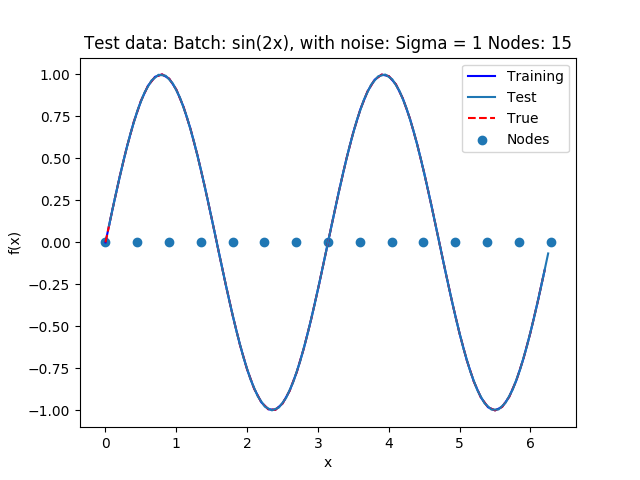
\includegraphics[width=1\textwidth]{plots/batch/best_sin2x.png}
        \caption{}
    \end{subfigure}
    \begin{subfigure}[t]{0.4\textwidth}
        \centering
        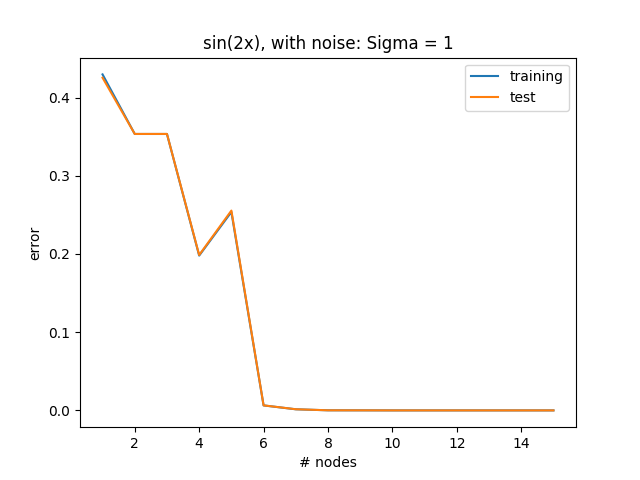
\includegraphics[width=1\textwidth]{plots/batch/best_sin2x_error.png}
        \caption{}
    \end{subfigure}
    \begin{subfigure}[t]{0.4\textwidth}
        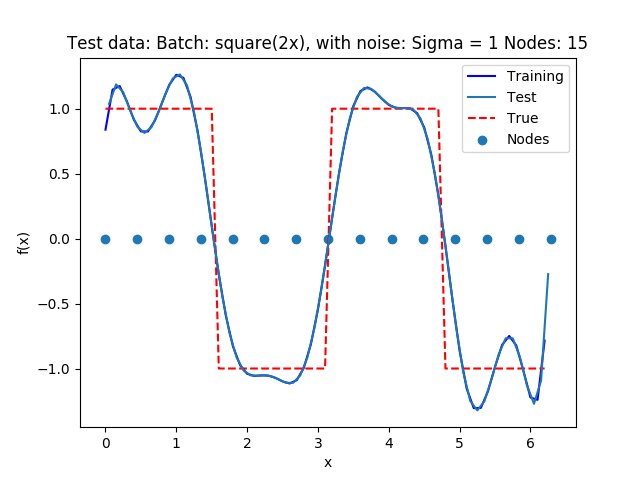
\includegraphics[width=1\textwidth]{plots/batch/best_square2x.png}
        \caption{}
    \end{subfigure}
    \begin{subfigure}[t]{0.4\textwidth}
        \centering
        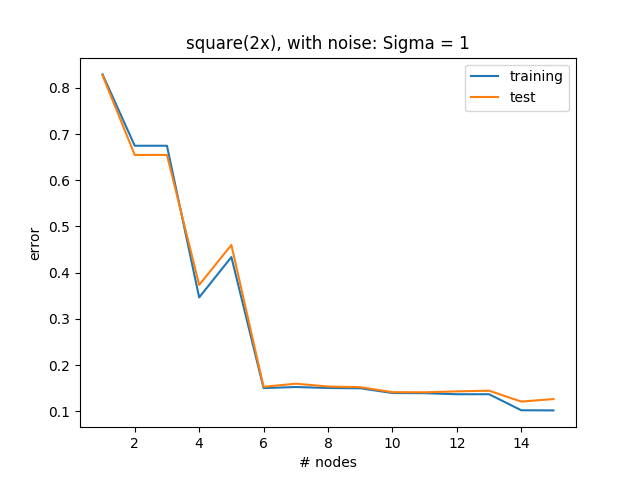
\includegraphics[width=1\textwidth]{plots/batch/best_square2x_error.png}
        \caption{}
    \end{subfigure}
\end{figure}

\begin{figure}[ht!]
  \centering
  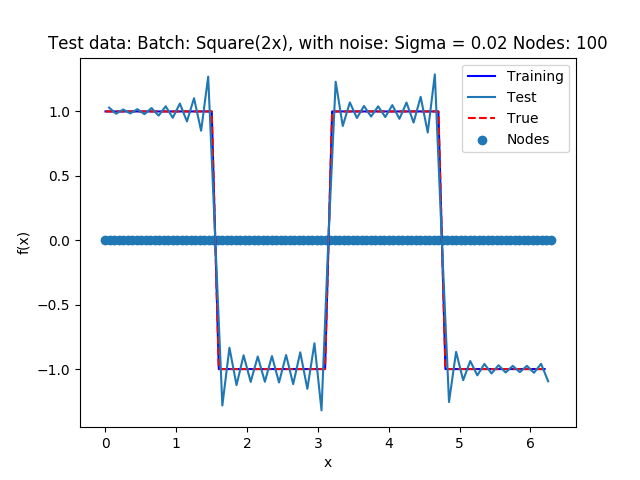
\includegraphics[width=0.5\linewidth]{plots/batch/best_square2x_extreme}
  \caption{test error 0.06}
  \label{}
\end{figure}

How can you simply transform the output of your RBF network to re- duce the residual error to 0 for the square(2x) problem? Still, how many units do you need? In what type of applications could this transform be particularly useful?

\begin{figure}[ht!]
    \centering
    \begin{subfigure}[t]{0.4\textwidth}
        \centering
        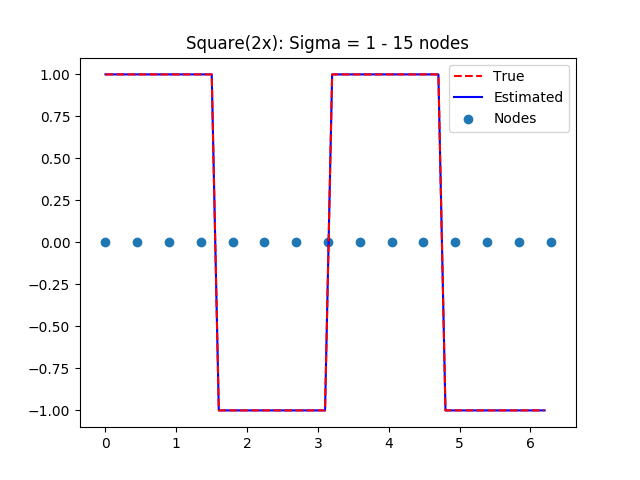
\includegraphics[width=1\textwidth]{plots/batch/best_square_cheat.png}
        \caption{}
    \end{subfigure}
    \begin{subfigure}[t]{0.4\textwidth}
        \centering
        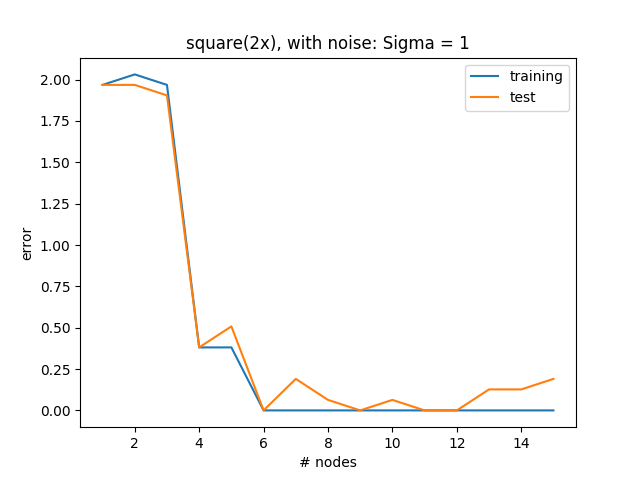
\includegraphics[width=1\textwidth]{plots/batch/square_error_sign}
        \caption{}
    \end{subfigure}
    \caption{Taking the sign of the estimated square function makes us reach 0 error with only 6 nodes.}
\end{figure}

\section{Regression with noise}
\FloatBarrier
Effect of altering sigma:
\FloatBarrier
\begin{figure}[ht!]
    \centering
    \begin{subfigure}[t]{0.4\textwidth}
        \centering
        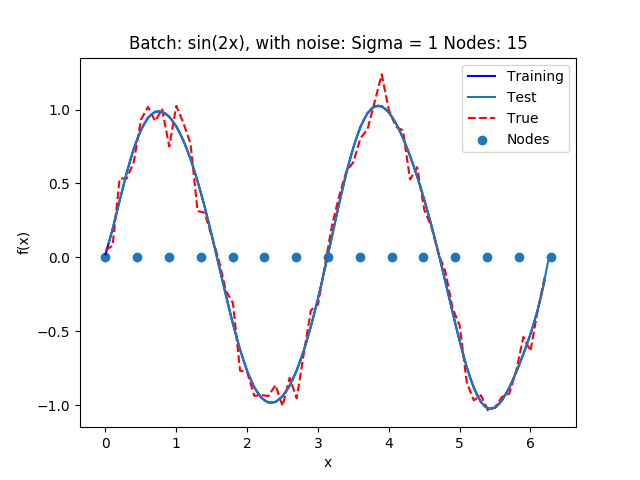
\includegraphics[width=1\textwidth]{plots/noise/batch_sin2x_sigma1.png}
        \caption{}
    \end{subfigure}
    \begin{subfigure}[t]{0.4\textwidth}
        \centering
        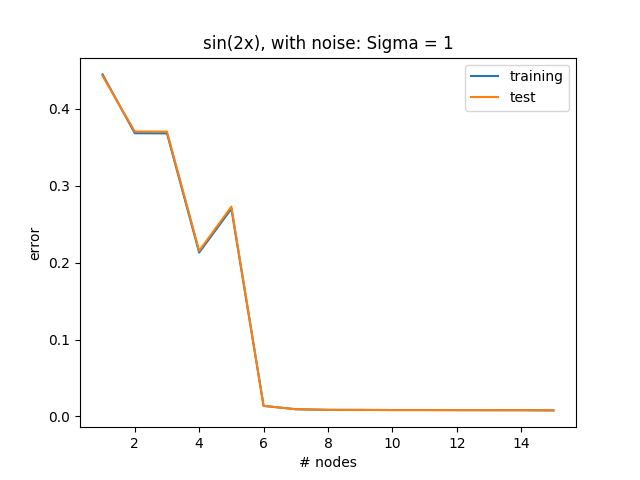
\includegraphics[width=1\textwidth]{plots/noise/batch_sin2x_error_sigma1.png}
        \caption{}
    \end{subfigure}
    \begin{subfigure}[t]{0.4\textwidth}
        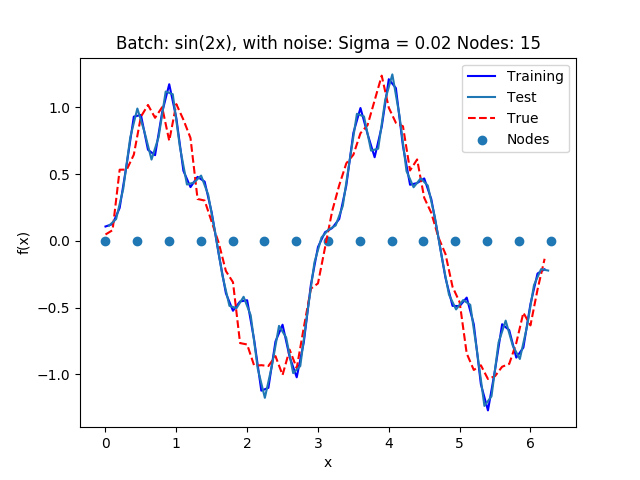
\includegraphics[width=1\textwidth]{plots/noise/batch_sin2x_sigma_002}
        \caption{}
    \end{subfigure}
    \begin{subfigure}[t]{0.4\textwidth}
        \centering
        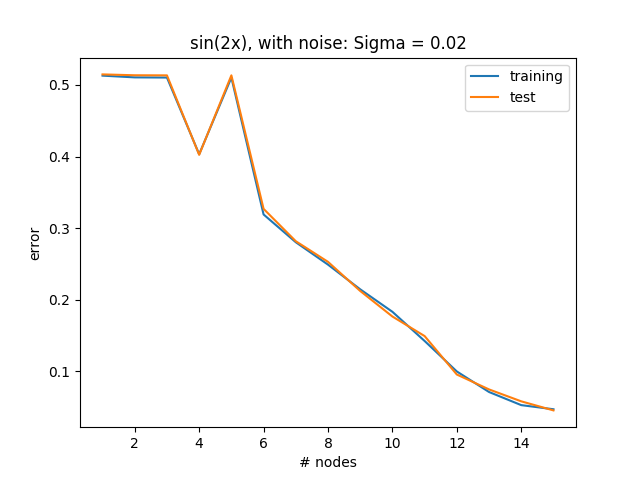
\includegraphics[width=1\textwidth]{plots/noise/batch_sin2x_error_sigma_002}
        \caption{}
    \end{subfigure}
    \caption{Plots of the effect of altering sigma on networks trained with batch method}
\end{figure}


\begin{figure}[ht!]
    \centering
    \begin{subfigure}[t]{0.4\textwidth}
        \centering
        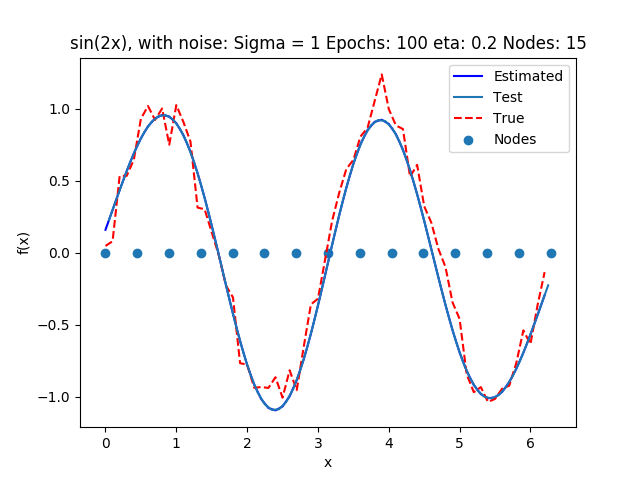
\includegraphics[width=1\textwidth]{plots/noise/seq_sin2x_100ep_sigma1}
        \caption{}
    \end{subfigure}
    \begin{subfigure}[t]{0.4\textwidth}
        \centering
        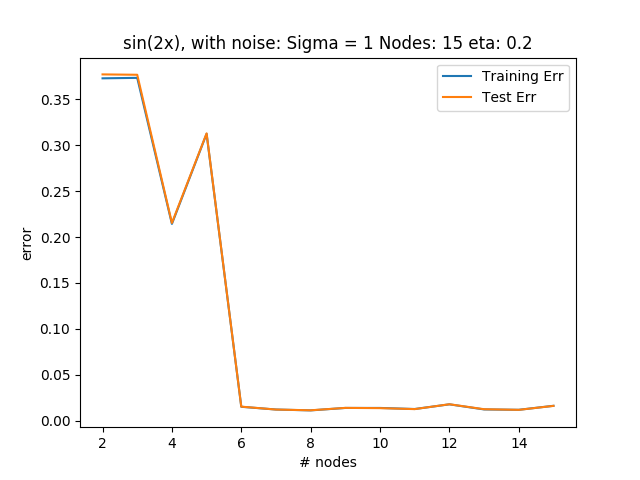
\includegraphics[width=1\textwidth]{plots/noise/seq_sin2x_100ep_sigma1_error}
        \caption{}
    \end{subfigure}
    \begin{subfigure}[t]{0.4\textwidth}
        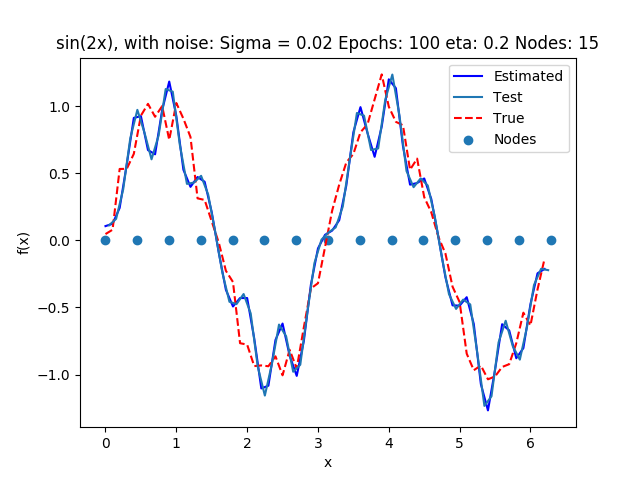
\includegraphics[width=1\textwidth]{plots/noise/seq_sin2x_100ep_sigma002}
        \caption{}
    \end{subfigure}
    \begin{subfigure}[t]{0.4\textwidth}
        \centering
        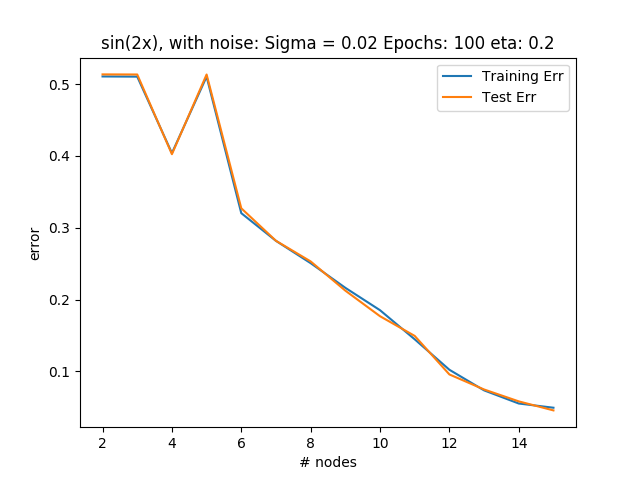
\includegraphics[width=1\textwidth]{plots/noise/seq_sin2x_100ep_sigma002_error}
        \caption{}
    \end{subfigure}
    \caption{Plots of the effect of altering sigma on networks trained with sequential method}
\end{figure}

Effect of number of epochs:

\begin{figure}[ht!]
    \centering
    \begin{subfigure}[t]{0.4\textwidth}
        \centering
        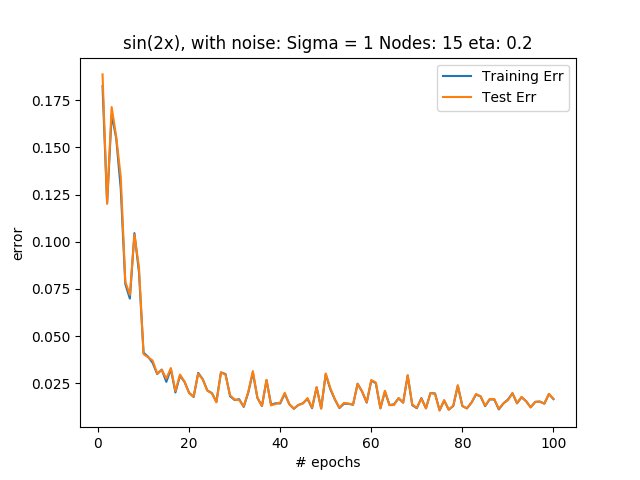
\includegraphics[width=1\textwidth]{plots/noise/seq_sin2x_15nodes_sigma1_error_per_epoch.png}
        \caption{}
    \end{subfigure}
    \begin{subfigure}[t]{0.4\textwidth}
        \centering
        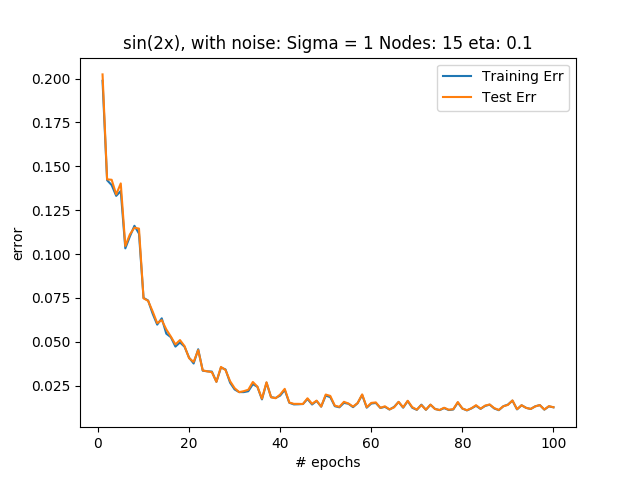
\includegraphics[width=1\textwidth]{plots/noise/seq_sin2x_15nodes_sigma1_error_per_epoch_eta01.png}
        \caption{}
    \end{subfigure}
    \begin{subfigure}[t]{0.4\textwidth}
        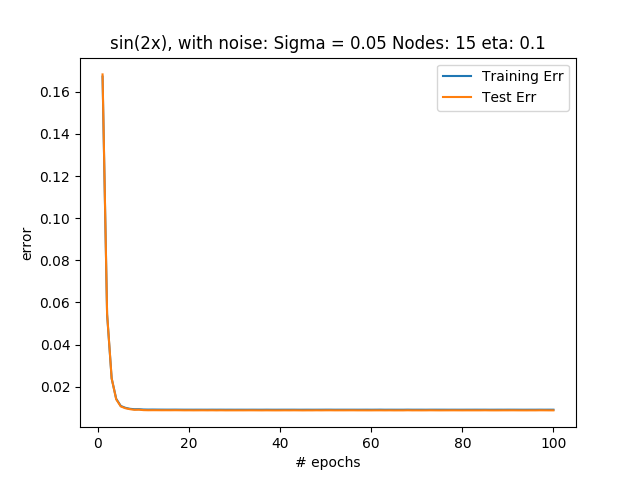
\includegraphics[width=1\textwidth]{plots/noise/seq_sin2x_15nodes_sigma1_error_per_epoch_eta005.png}
        \caption{}
    \end{subfigure}
    \begin{subfigure}[t]{0.4\textwidth}
        \centering
        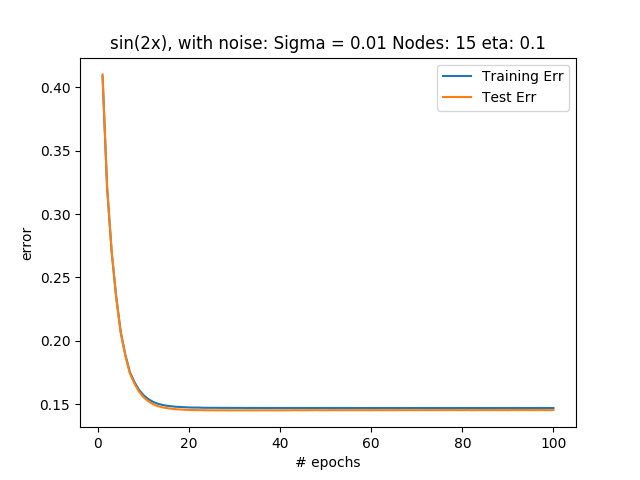
\includegraphics[width=1\textwidth]{plots/noise/seq_sin2x_15nodes_sigma1_error_per_epoch_eta001.png}
        \caption{}
    \end{subfigure}
    \caption{Plots of the error as a function of eta on networks trained with sequential method}
\end{figure}

\section{Competitive Learning}

\begin{figure}[ht!]
    \centering
    \begin{subfigure}[t]{0.4\textwidth}
        \centering
        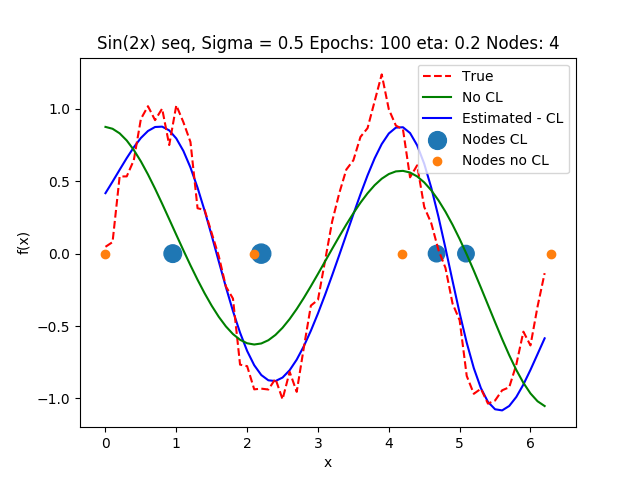
\includegraphics[width=1\textwidth]{plots/cl/sin2x_seq_CL_vs_no_cl_plots}
        \caption{Generated functions plotted with the node RBF node positions, with and without CL.}
    \end{subfigure}
    \begin{subfigure}[t]{0.4\textwidth}
        \centering
        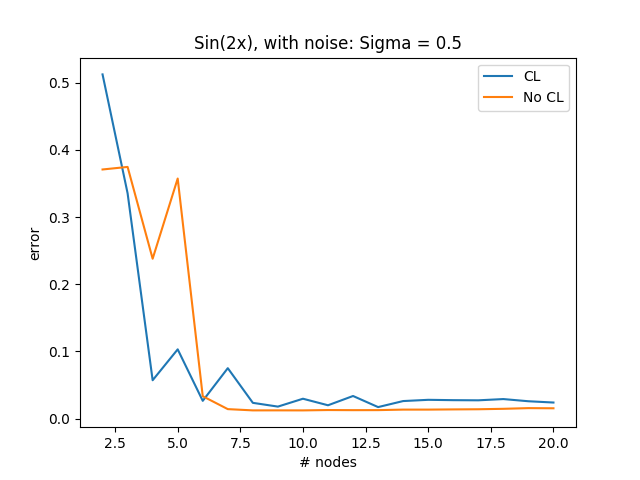
\includegraphics[width=1\textwidth]{plots/cl/sin2x_seq_CL_vs_no_cl_plots_error}
        \caption{Error as a function of the number of nodes, with and without competitive learning.}
    \end{subfigure}
    \caption{Plots of the effects of Cmpetitive Learning}
\end{figure}

\begin{figure}[ht!]
    \centering
    \begin{subfigure}[t]{0.4\textwidth}
        \centering
        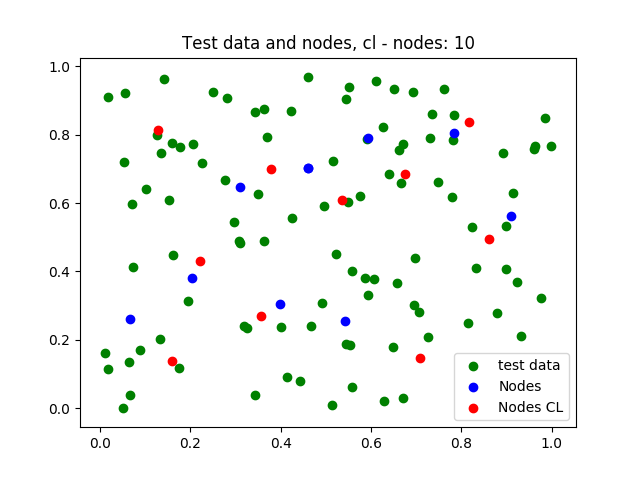
\includegraphics[width=1\textwidth]{plots/2d/input_basic_both_cl_batch_test}
        \caption{Test data and the node positions before and after competitive learning}
    \end{subfigure}
    \begin{subfigure}[t]{0.4\textwidth}
        \centering
        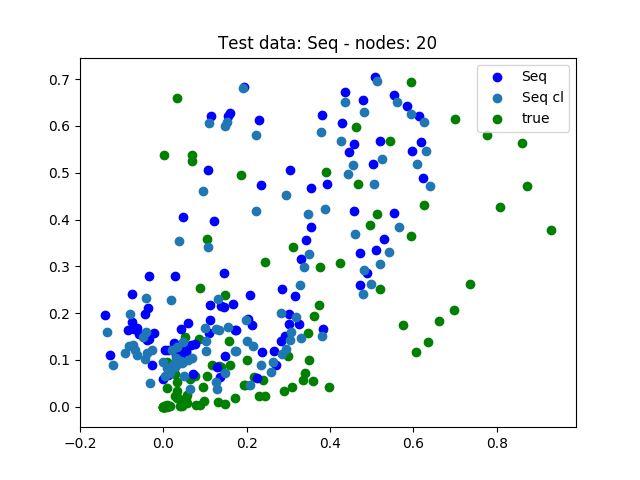
\includegraphics[width=1\textwidth]{plots/2d/first_basic_both_CL_output_seq_test_20_sigma25}
        \caption{Output of networks trained with and without competitive learning}
    \end{subfigure}
    \caption{}
\end{figure}

\end{document}
